\documentclass[12pt,spanish,a4paper, oneside, openany]{book}

\usepackage{graphicx}
\usepackage{setspace}	%double spacing for text, single for captions, footnotes, etc.
%\usepackage{hypernat} 	%substitut de cite que permet fer hyperlinks
% \usepackage{natbib}		% substituye a 'hypernat' que funciona en Windows.
\usepackage[square,sort,comma,numbers]{natbib}

\usepackage[utf8]{inputenc}
\usepackage[spanish]{babel}

\usepackage{lmodern} 
\usepackage{color}
\usepackage{hhline} 		% extended styles for tables
\usepackage{multirow}
\usepackage{subfigure}
\usepackage{acronym}
\usepackage{hyperref}
\usepackage{amsmath,amsmath,amssymb} 
\usepackage{fancyhdr}
\usepackage{epsfig, amsmath}
\usepackage{algorithm}
\usepackage{algorithmic}
\usepackage{pdflscape}
\usepackage[xindy]{glossaries} 
\usepackage{listings}

\renewcommand*{\bibfont}{\raggedright}

\selectlanguage{spanish}

% general settings
\hypersetup{
	linktocpage=true,
	colorlinks=true,
	linkcolor=blue,
	citecolor=blue,
}
\definecolor{Hgray}{gray}{0.6}

\newenvironment{definition}[1][Definition]{\begin{trivlist}
\item[\hskip \labelsep {\bfseries #1}]}{\end{trivlist}}

\setlength{\topmargin}{0cm}
\setlength{\textheight}{23cm}
\setlength{\textwidth}{17cm}
\setlength{\oddsidemargin}{0cm}
\setlength{\evensidemargin}{0cm}
\setlength{\headheight}{1cm}

\setlength{\parskip}{1em}

% indica que las 'sub-sub-sections' sean numeradas y aparezcan en el indice
\setcounter{secnumdepth}{3}
\setcounter{tocdepth}{2}

% settings for code
\renewcommand{\algorithmicrequire}{\textbf{Entrada: }}
\renewcommand{\algorithmicensure}{\textbf{Salida: }}

% glosario
\makeglossaries

% glossary
\newglossaryentry{em}{
	type=\acronymtype,
	name={EM}, 
	description={Esclerosis múltiple},
    first={esclerosis múltiple (EM)}
}

\newglossaryentry{snc}{
	type=\acronymtype,
	name={SNC}, 
	description={Sistema nervioso central},
    first={sistema nervioso central (SNC)}
}

\newglossaryentry{sban}{
	type=\acronymtype,
	name={SBAN}, 
	description={Sustancia blanca de apariencia normal},
    first={sustancia blanca de apariencia normal (SBAN)}
}

\newglossaryentry{sgan}{
	type=\acronymtype,
	name={SGAN}, 
	description={Sustancia gris de apariencia normal},
    first={sustancia gris de apariencia normal (SGAN)}
}

\newglossaryentry{sb}{
	type=\acronymtype,
	name={SB}, 
	description={Sustancia blanca},
    first={sustancia blanca (SB)}
}

\newglossaryentry{sg}{
	type=\acronymtype,
	name={SB}, 
	description={Sustancia gris},
    first={sustancia gris (SG)}
}

\newglossaryentry{rm}{
	type=\acronymtype,
	name={RM}, 
	description={Resonancia magnética},
    first={resonancia magnética (RM)}
}

\newglossaryentry{drm}{
	type=\acronymtype,
	name={dRM}, 
	description={Difusión por resonancia magnética},
    first={difusión por resonancia magnética (dRM)}
}

\newglossaryentry{dti}{
	type=\acronymtype,
	name={DTI}, 
	description={Tensor de difusión},
    first={tensor de difusión (DTI)}
}

\newglossaryentry{fa}{
	type=\acronymtype,
	name={FA}, 
	description={Anisotropía fraccional},
    first={anisotropía fraccional (FA)}
}

\newglossaryentry{md}{
	type=\acronymtype,
	name={MD}, 
	description={Difusividad media},
    first={difusividad media (MD)}
}

\newglossaryentry{ad}{
	type=\acronymtype,
	name={AD}, 
	description={Difusividad axial},
    first={difusividad axial (AD)}
}

\newglossaryentry{rd}{
	type=\acronymtype,
	name={RD}, 
	description={Difusividad radial},
    first={difusividad radial (RD)}
}

\newglossaryentry{csp}{
	type=\acronymtype,
	name={CSP}, 
	description={Common Spatial Pattern},
    first={``Common Spatial Pattern'' (CSP)}
}

\newglossaryentry{ann}{
	type=\acronymtype,
	name={ANN}, 
	description={Red neuroal artificial},
    firstplural={redes neuronales artificiales (ANN)}
}

\newglossaryentry{roi}{
	type=\acronymtype,
	name={ROI}, 
	description={Regiones de interés},
    firstplural={regiones de interés (ROI)}
}

\newglossaryentry{knn}{
	type=\acronymtype,
	name={K-NN}, 
	description={Algoritmo de los k-vecinos más cercanos },
    first={algoritmo de los k-vecinos más cercanos (K-NN)}
}

\newglossaryentry{cnn}{
	type=\acronymtype,
	name={CSP}, 
	description={Red neuronal convolucional},
    first={red neuronal convolucional (CNN)}
}

\newglossaryentry{frm}{
	type=\acronymtype,
	name={fRM}, 
	description={Resonancia magnética funcional},
    first={resonancia magnética funcional (fRM)}
}

\newglossaryentry{rbm}{
	type=\acronymtype,
	name={RBM}, 
	description={Retricted Bolzmann Machines},
    first={``Retricted Bolzmann Machines'' (RBM)}
}

\newglossaryentry{dbn}{
	type=\acronymtype,
	name={DBN}, 
	description={Deep Belief Network},
    first={``Deep Belief Network'' (DBN)}
}

\newglossaryentry{pca}{
	type=\acronymtype,
	name={PCA}, 
	description={Principal Component Analysis},
    first={``Principal Component Analysis'' (PCA)}
}

\newglossaryentry{ica}{
	type=\acronymtype,
	name={ICA}, 
	description={Independent Component Analysis},
    first={``Independent Component Analysis'' (ICA)}
}

\newglossaryentry{svm}{
	type=\acronymtype,
	name={SVM}, 
	description={Máquina de vector de soporte},
    firstplural={Máquinas de vector de soporte (SVM)}
}

\newglossaryentry{csv}{
	type=\acronymtype,
	name={CSV}, 
	description={del inglés ``comma-separated values''},
}
\makeglossaries

%%%%%%%%%%%%
% DOCUMENT %
%%%%%%%%%%%%
\begin{document}

% portada
%% portada
\newpage
\thispagestyle{empty}

\baselineskip 2em

%\vspace*{1cm}

\centerline {
\includegraphics[width=0.6\textwidth]{figs/UOC-logo}}
\begin{center}
\textsc{Universitat Oberta de Catalunya (UOC) \\
 Máster Universitario en Ciencia de Datos (\textit{Data Science})\\}

%\centerline {\pic{UOC}{4cm}}

\vspace*{1.5cm}

\textsc{\Large TRABAJO FINAL DE MÁSTER}


%\textbf{\Huge VirtualTechLab Model: }

\vspace*{1.5cm}

\textbf{\Large Aplicación de algoritmos de aprendizaje automático para predecir disfunción cognitiva en pacientes de esclerosis múltiple mediante índices de conectividad estructural}

%% \textbf{\large xxx subtítulo (en caso de existir) xxx}

\vspace{2.5cm}
\baselineskip 1em

\vspace{1cm}
\baselineskip 2em
-----------------------------------------------------------------------------\\
Autor:      Efraín Lima Miranda\\
Tutor:   Dr. Eloy Martínez de las Heras\\
Co-Tutor:   Dra. Sara Llufriu\\
Profesor: Dr. Jordi Casas Roma\\

-----------------------------------------------------------------------------\\
\vspace*{1.5cm}
Barcelona, \today

\end{center}



\newpage
\pagestyle{empty}
\hfill

%% copyright

\includegraphics[width=0.3\textwidth]{figs/previos/copyright.png}

Copyright © 2018 Efraín Lima Miranda

Esta obra está sujeta a una licencia de Reconocimiento-NoComercial-CompartirIgual 3.0

España de CreativeCommons (CC BY-NC-SA 3.0 ES) 

\url{http://creativecommons.org/licenses/by-nc-sa/3.0/es/}

\newpage

% ficha
\begin{center}

\textbf{FICHA DEL TRABAJO FINAL}

% Please add the following required packages to your document preamble:
% \usepackage{multirow}
\begin{table}[H]
\centering
\label{my-label}
\begin{tabular}{|r|l|}
\hline
\multirow{3}{*}{\textbf{Título del trabajo:}}          & Aplicación de algoritmos de aprendizaje automático   \\
                                                       & para predecir disfunción cognitiva en pacientes de   \\ 
                                                       & esclerosis múltiple mediante índices de conectividad \\
                                                       & estructural \\            
\hline
\textbf{Nombre del autor:}                             & Efraín Lima Miranda                                \\
\hline
\textbf{Nombre de los} & Dr. Eloy Martínez de las Heras                   \\ 
\textbf{colaboradores}  & Dra. Sara Llufriu                                 \\
                                                       \hline
\textbf{Nombre del PRA:}                               & Dr. Jordi Casas Roma                               \\ 
\hline
\textbf{Fecha de entrega:}                              & Junio de 2018 \\ 
\hline

\textbf{Titulación o programa:}                        & Máster Universitario en Ciencia de Datos (\textit{Data Science}) \\
\hline
\textbf{Área del Trabajo Final:}                       & Aprendizaje automático                                 \\ 
\hline
\textbf{Idioma:}                       & Español                                 \\ 

\hline
\textbf{Palabras clave:}                               & aprendizaje automático, conectividad estructural, \\
                                                       & esclerosis múltiple, rendimiento cognitivo \\ 
\hline

\end{tabular}
\end{table}

\null\vfill

\end{center}
\newpage


% dedicatoria
\thispagestyle{empty}

\parbox{0.6\textwidth}{\hspace{0.6\textwidth}}
\parbox{0.4\textwidth}{\bigskip\bigskip\bigskip\bigskip\bigskip\bigskip\bigskip\textit{ 
Dedicado a Laura, mi felicidad de cada día.
}}
\hfill
\newpage

% dedicatoria
\thispagestyle{empty}

\noindent
\textbf{\begin{Large}\textit{Agradecimientos}\end{Large}}
\newline
\newline
\noindent\textit{
Deseo expresar mi más sincero agradecimiento al tutor de este proyecto Dr. Eloy Martínez de las Heras por
sus apoyo personal y humano durante todo este trabajo.\\

A sí mismo, a todo el equipo del XXXX por su trabajo previo}

% resumen
\chapter*{Resumen}
\addcontentsline{toc}{chapter}{Resumen}
\onehalfspacing

\pagenumbering{roman} 
\setcounter{page}{1} 
\pagestyle{plain}
Este trabajo tiene como objetivo la predicción del rendimiento cognitivo del paciente con esclerosis múltiple (EM) a través de la cuantificación del volumen lesional y la microestructura de la red cerebral empleando herramientas de aprendizaje automático. Esta enfermedad neurodegenerativa es una de las causas más importantes de discapacidad física y cognitiva en adultos jóvenes.

Para esta investigación se ha dispuesto de una muestra de 182 sujetos, donde 140 padecen de EM y 42 son controles sanos. De cada uno de ellos se dispone de cuatro medidas de tensor de difusión (DTI) (Anisotropía fraccional, Difusividad media, Difusividad axial y Difusividad radial), número de fibras y volumen lesional. Toda esta información proveniente del análisis de la conectividad estructural  es presentada mediante matrices simétricas.

Tras realizar las tareas de preprocesamiento y limpieza de toda esta información, con el software NeuLoadData, se han estimado los mejores parámetros de configuración para los algoritmos ``Logistic Regression'', ``Support Vector Machine (SVM)'', ``Gaussian Naive Bayes, Random Forest Classifier'' y ``Artificial Neural Network (ANN)''. Usando únicamente las medidas de tensor de difusión todos los modelos obtenidos han sido capaces de predecir exitosamente más del 75\%. Por lo tanto, el enfoque propuesto de aprendizaje automático para la predicción el rendimiento cognitivo en pacientes con EM ha demostrado su utilidad e interés como herramienta para analizar un gran conjunto de datos satisfactoriamente en el campo sanitario.

\vspace*{1cm}

\textbf{Palabras clave:} aprendizaje automático, conectividad estructural, esclerosis múltiple, rendimiento cognitivo

% abstract
%\chapter*{Abstract}
%\addcontentsline{toc}{chapter}{Abstract}
%\onehalfspacing
%\vspace*{1cm}
The present study aims to predict the cognitive performance of patients with multiple sclerosis (MS) through quantification of lesional volume and the microstructure of the brain network by means of machine learning techniques. This neurodegenerative disease is one of the main causes of both physical and cognitive disability in young adults.

For this research, we have a sample of 140 patients with Multiple Sclerosis and 42 healthy controls. For each participant, information relating to four measures of diffusion tensor (DTI) (fractional anisotropy, medium diffusivity, axial diffusivity and radial diffusivity), number of fibers and lesional volume has been recorded. All this information coming from the analysis of structural connectivity is presented by symmetric matrices.

After carrying out preprocessing tasks on all of this information using the NeuLoadData software, the best configuration parameters have been estimated for the algorithms Logistic Regression, Support Vector Machine (SVM), Gaussian Naive Bayes, Random Forest Classifier and Artificial Neural Network (ANN). Making use of only diffusion tensor measurements, all the models have had a successful prediction rate of over 75\%. Therefore, the proposed approach of machine learning for prediction cognitive performance in patients with MS has demonstrated satisfactorily its usefulness and interest as a tool to analyze a large set of data in the health field.

\textbf{Keywords:} manchine learning, structural connectivity, multiple sclerosis, cognitive performance


\pagestyle{fancy}
\renewcommand{\chaptermark}[1]{ \markboth{#1}{}}
\renewcommand{\sectionmark}[1]{\markright{ \thesection.\ #1}}
\lhead[\fancyplain{}{\bfseries\thepage}]{\fancyplain{}{\bfseries\rightmark}}
\rhead[\fancyplain{}{\bfseries\leftmark}]{\fancyplain{}{\bfseries\thepage}}
\cfoot{}

% indice
\cleardoublepage
\phantomsection
\addcontentsline{toc}{chapter}{Índice}
\tableofcontents

% listado de figuras
\cleardoublepage
\phantomsection
\addcontentsline{toc}{chapter}{Listado de Figuras}
\listoffigures

% listado de tablas
\cleardoublepage
\phantomsection
\addcontentsline{toc}{chapter}{Listado de Tablas}
\listoftables

% Acronyms
\printglossary[title=Acrónimos, type=\acronymtype]

\thispagestyle{empty}

\pagenumbering{arabic}

\pagestyle{fancy}
\renewcommand{\chaptermark}[1]{ \markboth{#1}{}}
\renewcommand{\sectionmark}[1]{\markright{ \thesection.\ #1}}
\lhead[\fancyplain{}{\bfseries\thepage}]{\fancyplain{}{\bfseries\rightmark}}
\rhead[\fancyplain{}{\bfseries\leftmark}]{\fancyplain{}{\bfseries\thepage}}
\cfoot{}

\onehalfspacing

% PROLEGÓMENO
\part{Prolegómeno}
\null\vfill
\chapter{Introducción}
\label{chapter:introduccion}

La \gls{em} es una enfermedad neurodegenerativa crónica, inflamatoria y desmielinizante del \gls{snc}, de carácter autoinmune y considerada como una de las causas más importantes de discapacidad física y cognitiva en adultos jóvenes \cite{Rocca2015ClinicalSclerosis}. Esta enfermedad se caracteriza principalmente por la presencia de placas desmielinizadas focales, y por una afectación microestructural difusa más allá de las lesiones en la gls{sban} y la \gls{sgan}. Ambos componentes son los responsables de la atrofia cerebral y, en cierta medida, están asociados con la discapacidad cognitiva \cite{Kutzelnigg2014PathologyDiseases}. Este deterioro cognitivo está presente en el 40-70\% de los pacientes, incluso durante etapas tempranas de la enfermedad. Los déficits cognitivos más comunes son los relacionados con la atención, las funciones ejecutivas, la velocidad de procesamiento de la información y la memoria episódica \cite{Chiaravalloti2008CognitiveSclerosisb}. 

La \gls{rm} convencional ha demostrado ser una  técnica útil para el diagnóstico y monitorización de la enfermedad de \gls{em}.  La presentación de lesiones características de la enfermedad se muestran hipointensas en secuencias potenciadas en T1 y con un aumento de señal en secuencias potenciadas en T2. Sin embargo, la presencia de lesiones y las manifestaciones clínicas de los pacientes son modestas \cite{Barkhof2002TheRevisited}. Probablemente, a causa de la baja especificidad en la patología subyacente y a la baja sensibilidad del daño del tejido de apariencia normal en este tipo de secuencias.  La existencia de nuevas modalidades de imagen por RM, denominadas \gls{rm} avanzada o no convencional, ha aportado información más sensible más allá de las lesiones focales, permitiendo estudiar el tejido de apariencia normal, siendo una de las modalidades más populares actualmente es la \gls{drm}. Esta técnica de \gls{rm} se basa en el estudio del movimiento de las moléculas de agua y permite caracterizar las trayectorias de \gls{sb} de forma no invasiva, dado que en la \gls{sb} este movimiento de moléculas de agua predomina en la dirección paralela al axón y se encuentra limitado en su dirección perpendicular \cite{Basser2000InDatab}.  Por tanto, a partir de la \gls{drm} podemos obtener datos cuantitativos y patológicamente más específicos capaces de detectar cambios en la integridad microestructural en \gls{sban} y \gls{sgan}. A partir de la \gls{drm} podemos obtener unas medidas que se conocen como \gls{dti}. Estas medidas cuantifican la direccionalidad y magnitud del movimiento de las moléculas de agua en el espacio tridimensional. Dado que existe una fuerte direccionalidad debido a la presencia de mielina y axones en la \gls{sb}, el movimiento es anisotrópico y puede representarse como una elipsoide, donde el semieje principal indica la máxima difusividad. La elipsoide se puede parametrizar por un conjunto de vectores y valores propios que nos proporcionan unos índices sensibles a la integridad del tejido. El más común es la \gls{fa}. La \gls{fa} es una variable numérica cuyos valores oscilan entre 0 (máxima isotropía) y 1 (máxima anisotropía). La \gls{fa} es mayor en la \gls{sb} que en la \gls{sg}, debido a que la movilidad del agua está altamente influenciada por la organización de las fibras nerviosas. Por este motivo, el valor de \gls{fa} es comúnmente utilizado en los estudios como un marcador de la integridad estructural, ya que la pérdida de barreras reduce el grado de anisotropía (menor \gls{fa}). Hay otros valores del tensor que se pueden cuantificar como: la \gls{md}, la \gls{ad} y la \gls{rd}. Mientras que la \gls{fa} y la \gls{md} se han asociado a diversos cambios patológicos en el tejido, los cambios de \gls{ad} y \gls{rd} se han asociado con daño axonal y desmielinización principalmente en estudios con modelos animales \cite{Song2005DemyelinationBrain}.

Mediante el tensor de difusión es posible generar una representación de las fibras de la \gls{sb} o tractografía. La tractografía utiliza la dirección de máxima difusividad entre vóxeles cercanos para trazar las diferentes conexiones que componen la red cerebral. Sin embargo, esta aproximación es muy simplista dado que el modelo por \gls{dti} no es capaz de descomponer las diferentes fibras contenidas en un solo vóxel. La estructura local de la SB presenta regiones de cruce, dobleces o dispersión de fibras en más del 90\% de los vóxeles \cite{Jeurissen2013InvestigatingImaging}, El uso de modelos avanzados de tractografía proporciona una representación de mayor resolución angular de los diferentes máximos locales contenidos dentro del vóxel y reemplaza la representación de la elipsoide por otra estimación más compleja \cite{Tuch2002HighHeterogeneity}. Gracias a esto se puede descomponer las fibras de \gls{sb} en diferentes direcciones en una región de cruce de fibras y reconstruir aquellos tractos que presentan una gran curvatura y una baja \gls{fa} \cite{Martinez-Heras2015ImprovedRadiation}.  

La realización de la modelos avanzados de tractografía permite generar fibras de \gls{sb} biológicamente más precisas respecto a la anatomía subyacente y trazar las trayectorias que componen la red cerebral \cite{Rubinov2010ComplexInterpretations}. Una vez generada la  tractografía es posible cuantificar la reconstrucción con diferentes índices como pueden ser el número de fibras, el volumen lesional de las conexiones o las medidas del tensor. Esto puede facilitar el uso de medidas sensibles para diferenciar entre un cerebro sano y otro con presencia de una patología. Además de la posibilidad de detectar qué conexiones del cerebro (subsistemas) guardan algún tipo de relación con variables clínicas de interés \cite{Llufriu2017StructuralSclerosis}. 

A través de la cuantificación de este tipo de medidas sensibles a la microestructura tisular se pueden relacionar cambios patológicos de la \gls{sban} con el deterioro cognitivo en pacientes con \gls{em} \cite{Gabilondo2014Trans-synapticSclerosis} \cite{Llufriu2017StructuralSclerosis}. Otra herramienta útil para la detección de anomalías de la red cerebral es la teoría de grafos \cite{Bullmore2009ComplexSystems}. Esta metodología permite caracterizar varios aspectos de la estructura de la red, designando las distintas regiones de interés (\gls{sg}) como nodos de un grafo y las conexiones entre estos nodos como aristas (\gls{sb}). Este planteamiento ha facilitado la comprensión de la arquitectura de la red cerebral. Basándose en estos métodos, estudios recientes han demostrado que el cerebro no puede ser considerado simplemente como una gran red interconectada, sino más bien una colección jerárquica de redes de ámbito local que cooperan paralelamente y son capaces de optimizar información por medio de diferentes estructuras modulares \cite{Sporns2011NetworksBrain}. 

El uso de herramientas de análisis de la conectividad estructural en los pacientes con \gls{em} ha demostrado que la red cerebral de estos pacientes tienen una menor capacidad para intercambiar y procesar información eficazmente. Además, la existencia de mecanismos de desconexión ha sido descrita como una causa importante en la manifestación de la alteración cognitiva en la \gls{em} \cite{Shu2011DiffusionSclerosis} \cite{Llufriu2017StructuralSclerosis} \cite{Bozzali2013AnatomicalSclerosis} \cite{Louapre2014BrainStudy} \cite{Dineen2009DisconnectionSclerosis}. Sin embargo, a pesar de estos importantes hallazgos, hay que tener en cuenta otros factores que pueden relacionarse con el rendimiento cognitivo como el volumen lesional y el daño tisular local de la \gls{sb} \cite{Stellmann2017ReducedMS} \cite{Ouellette2018LesionSclerosis.}. 

Como herramienta de análisis de este trabajo se introduce el aprendizaje automático para el estudio de la conectividad estructural de los pacientes con \gls{em}. El aprendizaje automático forma parte de las ciencias computacionales caracterizándose por la búsqueda de modelos capaces de generalizar comportamientos implícitos en los datos haciendo que "aprendan" automáticamente a partir de la información proporcionada. La tarea de clasificación es una de las más importantes entre todo el conjunto de algoritmos que se engloban en las técnicas de aprendizaje automático. Utilizando algoritmos supervisados, se caracteriza por la búsqueda de un modelo capaz de asignar un conjunto de clases, o etiquetas, basándose en la información contenida en los datos. Estas técnicas de aprendizaje automático han ayudado a numerosos estudios a obtener resultados muy positivos, como por ejemplo, a la hora de diferenciar entre pacientes con \gls{em} y sujetos sanos basándose en la información contenida en las imágenes de \gls{rm} \cite{Zhang2016ComparisonMachine}.




% DESARROLLO
\part{Desarrollo}
\null\vfill
\chapter{Desarrollo del trabajo}
\label{chapter:desarrollo}
Los métodos del aprendizaje automático pueden ayudar a las deficiencias de la interpretación humana en relación con la complejidad del cerebro [1]. Más concretamente, usando algoritmos supervisados de clasificación predecir la disfunción cognitiva en pacientes de \gls{em}

Teniendo siempre presente esta meta, se ha llevado a cabo un estudio preliminar de los datos proporcionados. Posteriormente se implementó un sistema para la limpieza y preparación de los datos para la aplicación a los algoritmos de aprendizaje automático. Con especial énfasis en descartar modelos que sufrieran sobreajuste y usando de métodos de validación cruzada y remuestreo se han validado los resultados obtenidos siguiendo métricas de exactitud o ``accuracy''.

\chapter{Estudio de los datos}
\label{chapter:estudio}
A través de un convenio de cooperación entre la Universidad Oberta de Catalunya y el Institut d'investigacions Biomèdiques August Pi i Sunyer (IDIBAPS) [2], contamos con datos clínicos y de neuroimagen avanzada de personas que padecen esclerosis múltiple junto con un grupo control.

Como información clave para este estudio destacan las matrices simétricas de conectividad estructural. Estas matrices son el resultado del procesado de imágenes de \gls{drm}. Los índices obtenidos a través de estas técnicas, tales como las medidas del tensor, el número de fibras y el volumen de lesión pueden facilitar la obtención de medidas sensibles para diferenciar entre un paciente con un mejor o peor rendimiento cognitivo:

\begin{description}
 \item [\gls{dti}-\gls{fa}] Anisotropía fraccional
 \item [\gls{dti}-\gls{md}] Difusividad media
 \item [\gls{dti}-L1] Difusividad axial
 \item [\gls{dti}-RX] Difusividad radial
 \item [RAW] Número de fibras
 \item [LS] Volumen lesional
\end{description}


(PEC3) Los pacientes presentan un peor rendimiento cognitivo principalmente en atención y memoria. Para detectar una posible discapacidad cognitiva de los pacientes hemos realizado una evaluación neuropsicológica. Esta evaluación incluye una batería (Brief Repeatable Battery, BRBN [3]) junto con otras prueba cognitivas. Los dominios estudiados han sido los relacionados con aprendizaje y memoria. En la siguiente tabla podemos observar el número de pacientes cuya discapacidad está por debajo de puntuaciones -1 y -2 desviaciones estándares por debajo de una población de referencia (ver Tabla 1).

(Tabla sumas)

\section{Distribución de los datos}

La información proveída por el grupo de Imagen Avanzada en enfermedades Neuroinmunológicas (ImaginEM) \cite{QueNeuroinmunologia} se encuentra organizada en una hoja de cálculo donde se presentan los datos clínicos de cada paciente anonimizado y una estructura en forma de distintos directorios donde se presentan cada matriz de adyacencia.

\subsection{Hoja de cálculo (Indice principal)}
La hoja del cálculo con los datos de cada paciente consta de 255 filas, una por paciente
y 33 columnas. Entre ellas se encuentra la columna $profile$ con los siguientes valores:

\begin{description}
\item [none] Persona con \gls{em} sin deficiencia cognitiva detectada.
\item [HV] Persona sin \gls{em}
\item [memory] Persona con \gls{em} y afectación en memoria
\item [attention] Persona con \gls{em} y afectación en atención.
\item [mem\_att] Persona con \gls{em} y deterioro cognitivo en memoria y atención.
\end{description}

\subsection{Directorios con matrices}
Estos directorios siguen un formato establecido donde cada fichero indica en su prefijo a qué paciente corresponde y, en función del directorio donde se encuentra, la medición de dónde proviene la matriz. Por ejemplo, el fichero situado en
\begin{lstlisting}
FIS/ADJACENCY_MATRICES_GRAPH/DTI_indices/FA/FIS_001_FA.csv
\end{lstlisting}
corresponde con la medida DTI-\gls{fa} del paciente de cuyo identificador es FIS\_001. En la tabla 2 se describe detalladamente esta estructura.

Cada fichero que contiene los valores de una matriz está almacenado en formato \gls{csv} conteniendo todos ellos 76 filas y 76 columnas sin ningún valor nulo o vacío.

(Tabla 2: Organización directorios)

\section{Características de los datos}
Para cada instancia que disponemos de los datos, contamos con seis matrices de adyacencia de tamaño 76x76. Aparte de estas matrices los valores de estas matrices, de la hoja de cálculo se presentan 33 columnas. Es decir, disponemos ejemplares de la muestra con hasta (TODO formula)  $76 x 76 x 6 + 33 = 34689$ atributos cada uno. 

Los valores de las matrices son completos, es decir, si una instancia tiene una matriz, todos sus valores están presentes. Como se ve en la tabla1-TODO, no todas las instancias tienen todas sus matrices. También se encuentran X matrices ``perdidas'', sin correspondencia con ninguna instancia de la hoja de cálculo y, por lo tanto, descartadas para el estudio. 


\chapter{Software para el preprocesado}
\label{chapter:preprocesado}
El preprocesamiento de los datos es la etapa encargada de la limpieza de los datos, la integración en el sistema de aprendizaje automático, la transformación y reducción para los algoritmos de aprendizaje automático. Después de esta fase, los datos deben de ofrecerse a través de una fuente consistente y adecuada para la aplicación de los diferentes algoritmos de aprendizaje automático.

Con esta finalidad se ha desarrollado el software NeuLoadData. Usando como origen los archivos contenidos en los directorios anteriormente descritos y su correspondiente hoja de cálculo es capaz de limpiar, validar e integrar los datos para su posterior uso.

\subsection{NeuLoadData}
Este software ha sido concebido especialmente para los datos en el formato proporcionado por IDIBAPS para este estudio. Aún así, su implementación se ha centrado en un enfoque genérico para su posible adaptación a nuevos orígenes de datos o necesidades futuras.

Usando Python como lenguaje de programación se ha implementado esta herramienta y publicado para la comunidad bajo licencia Open Source en la plataforma de desarrollo colaborativo Github \cite{WhatGitHub.} bajo la dirección \url{https://github.com/efrain70/NeuDataLoad}.

\subsubsection{Metodología de desarrollo}

La implementación se ha ejecutado siguiendo una metodología iterativa basada en los principios del Manifiesto por el Desarrollo Ágil de Software \cite{ManifiestoSoftware}. Principalmente, a medida que se aparecían las necesidades sobre el conjunto de datos, se han añadido nuevas funcionalidades completas y dispuesto para su utilización.

\subsubsection{Aseguramiento de la calidad}
La calidad de este software es clave para una correcta utilización de los datos en todo el proceso de investigación. Cualquier error en el preprocesado podría dar a valores inesperados en los resultados o condicionar la investigación hacia erróneamente.

Con este propósito, se ha desarrollado todo este software validando todo su funcionamiento a través de pruebas unitarias y de integración. Para ello se ha usado la herramienta py.test \cite{Pytest:Documentation} junto con la plataforma Coveralls \cite{CoverallsStatistics} (dirección del proyecto \url{https://coveralls.io/github/efrain70/NeuDataLoad} imagen 2) para controlar que la cobertura del código validado con estas pruebas siempre es total, 100\%.

No solamente ha comprobado que el código funciona correctamente, también que su sintaxis se ajusta con los estándares del lenguaje. Para ello se ha validado el estilo de todo el código bajo la guía especial para Python PEP8 \cite{PEPPython.orgb} y para la documentación en código PEP257 \cite{PEPPython.org} y controlado la complejidad del mismo.

Para ejecutar todo estas validaciones de la calidad del software en un entorno ágil, se ha  configurado el proceso siguiendo un enfoque de integración continua, usando para ello pipelines de la plataforma Travis CI \cite{TravisConfidence} (Dirección del proyecto \url{https://travis-ci.org/efrain70/NeuDataLoad}, imagen 1) como plataforma coordinada con el repositorio Github. Esto implica que cada vez que se publique alguna modificación en el código, Github se coordina con Travis CI para la ejecución de todas las pruebas anteriormente descritas reportando los posibles errores automáticamente.

\subsubsection{Documentación}
Toda la documentación de este software se ha descrito usando la tecnología propia del lenguaje de Python. Gracias a la utilidad de Sphinx \cite{OverviewDocumentation} se han generado automáticamente la documentación con el contenido descrito en el código. Toda esta documentación del software se ha incluido en el código y generado en formato web para su publicación en Github Pages \cite{GitHubLive.}. Bajo la dirección \url{https://efrain70.github.io/NeuDataLoad/}, imagen 3, se encuentra la interfaz de la aplicación detallada.

\subsubsection{Funcionalidades principales}
Las funcionalidades principales implementadas en software son:

Aplicación de transformaciones a las matrices:
Para adaptarse a las necesidades de los algoritmos de aprendizaje automático y para mejorar su rendimiento se incluyen un conjunto de herramientas para la transformación de las matrices:

Combinación de las matrices: teniendo como entrada un conjunto de matrices del mismo tamaño NxM, se le aplica una función a las celdas de todas las matrices situadas en las mismas coordenadas i,j dando como resultado una nueva de tamaño NxM con los resultados de la aplicación de la función.

Aplanamiento o remodelación: A partir de una matriz de tamaño NxM, se generan una nueva de una única dimensión con los valores extendidos. Es decir, obtendremos N·M atributos nuevos.

Binarización: a partir de un valor de frontera, la matriz convierte todos sus valores a 1 y 0 dependiendo si éstos superan el valor de frontera. Es decir, se obtiene una matriz con valores binarios de tamaño NxM.

Selección de los atributos: Selección de atributos del conjunto de datos y de los posibles nuevos atributos generados durante la transformación aplanamiento. 

Todas estas funcionalidades se implementan principalmente en el módulo ‘utils’, pero puede ser usada a través de la clase NeuProfiles directamente o por medio de transformadores de para pipelines de scikit-learn \cite{Scikit-learn:Documentation}. En el módulo transformer están las clases transformadoras (\url{https://efrain70.github.io/NeuDataLoad/transformer.html}) que facilitan la integración en el framefork scikit-learn.

Carga automática y validación de las matrices
Usando través de la ruta local o remota introducida por el usuario, NeuLoadData valida las matrices leídas de los ficheros y las incluye en un único dataframe, contenedor de toda la información de la hoja de cálculos y las matrices de adyacencia.

NeuProfiles es clase que implementa esta funcionalidad a través de su método load, dando como resultado objeto contenedor dataframe de Pandas \cite{PythonLibrary} conjuntamente con las utilidades para la transformaciones de matrices. (\url{https://efrain70.github.io/NeuDataLoad/profiles.html})



\chapter{Algoritmos de aprendizaje automático}
\label{chapter:algoritmos}
El aprendizaje automático es una rama de la inteligencia artificial cuyo objetivo es proporcionar técnicas para hacer que los sistemas “aprendan”. Este aprendizaje se basa en algoritmos que a partir de un conjunto de datos son capaces de crear un modelo capaz de generalizar comportamientos y reconocer patrones. Estos modelos se caracterizan por su finalidad y se clasifican en dos grupos diferenciados: Algoritmos supervisados y algoritmos no supervisados

\section{Tipos de tareas}
En función de la tarea que queramos resolver con el aprendizaje automático podemos diferenciar en tres grupos: clasificación, regresión y agrupamiento. Todas ellas siguen un paradigma inductivo donde, a partir de los datos y un modelo se puede obtener un nuevo conocimiento que puede ser aplicado posteriormente a nuevos datos. A su vez, éstos se diferencia en dos grandes grupos, algoritmos supervisados y no supervisados. 

\subsection{Clasificación}
La tarea de clasificación se centra en asignar un conjunto de clases a instancias de un dominio compuesto por atributos discretos o continuos. Estas clases, o etiquetas, tiene que ser conocidas para un subconjunto para la construcción del modelo.

\subsection{Regresión}
La tarea de regresión la podemos describir como una clasificación con clases continuas. Es decir, asigna un valor numérico a instancias de un dominio compuesto por atributos discretos o continuos. Este modelo está definido por una función, generalmente desconocida, que establece un valor numérico para los nuevos datos.

\subsection{Agrupamiento}
El agrupamiento, al igual que la clasificación y la regresión, es una tarea inductiva. En cambio, se considera un algoritmo no supervisado ya que no se dispone de un conjunto de clases para predecir. El resultado del agrupamiento es un conjunto de clases y la asignación de cada elemento del conjunto de datos a una de estas clases basándose en la similitud entre las instancias. El modelo que se obtiene como resultado del agrupamiento también asigna a cada nueva instancia una clase de las anteriormente obtenidas.

\section{Algoritmos supervisados y algoritmos no supervisados}

\subsection{Algoritmos supervisados}
Estos algoritmos requieren un conjunto de datos etiquetados. Si las etiquetas de los datos son categóricos se denominan algoritmos de clasificación. En cambio, si son etiquetas numéricas corresponden a algoritmos de regresión. Por lo tanto, son usados tanto en tareas de clasificación como de regresión.

\subsection{Algoritmos no supervisados}
Estos algoritmos no necesitan que los datos dispongan de ninguna etiqueta o clasificación previa. Se centran en el agrupamiento o segmentación con el fin de encontrar características  similares. Podemos diferenciar entre  dos grupos; los métodos jerárquicos donde se obtiene una organización con varios niveles de agrupación, y los métodos particionales o no jerárquicos.


\chapter{Experimentos}
\label{chapter:experimentos}
En este trabajo nos hemos centrado principalmente en la aplicación de algoritmos de clasificación de aprendizaje supervisado para las etiquetas relacionadas con las disfunciones cognitivas presentes en los datos proporcionados. Los experimentos que se ha llevado persiguen el objetivo de obtener el mejor modelo para cada algoritmos a partir de un conjunto de datos usados para su entrenamiento.



\chapter{Resultados}
\label{chapter:resultados}
Una vez que obtenemos para cada algoritmos la mejor combinación de resultados, se ejecutan los modelos calculados con el conjunto de test y de entrenamiento inicial. De esta forma se pretende estimar el sobreajuste, ``overfitting'', del modelo. 

\section{Concepto de sobreajuste}
\label{section:sobreajuste}
El sobreajuste u ``overfitting'' se produce cuando un modelo cuando obtiene muy buenos resultados bien con los datos de entrenamiento, pero su precisión es notablemente más baja con el conjunto de test. Esto se produce porque el modelo se ha adaptado a los valores del conjunto de entrenamiento y no es capaz de generalizar para datos que no ha procesado. En la imagen \ref{figure:sobreajuste} podemos observar gráficamente en que consiste este problema.

\begin{figure}[H]
\centering
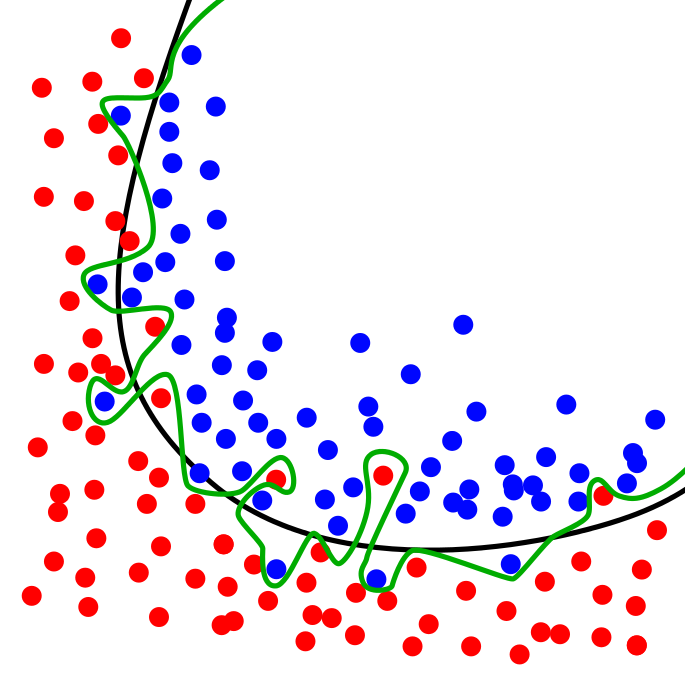
\includegraphics[width=0.3\textwidth]{figs/Overfitting.png}
\caption{Ejemplo de sobreajuste, línea verde \cite{SobreajusteLibre}}
\label{figure:sobreajuste}
\end{figure}

Este sobreajuste está directamente relacionado con la complejidad del modelo, cuanto más complejo sea más tendencia tendrá a sobreajustarse. Aparte, si el conjunto de datos del que disponemos es reducido, como en nuestro caso, este problema de sobreajuste estará muy presente.

\section{Resumen de los resultados}

En la tabla \ref{table:resultados} podemos ver para cada algoritmo los resultados obtenidos cuando se ejecuta la mejor configuración obtenida en los pasos anteriores. Entre los resultados se distinguen los valores para el conjunto de entrenamiento y para el conjunto de test. De esta forma controlamos el sobreajuste anteriormente descrito.


\begin{table}[H]
\centering
\begin{tabular}{c|c|c|c|c|}
\cline{2-5}
                                        & \multicolumn{2}{c|}{\textbf{Todas las matrices}} & \multicolumn{2}{c|}{\textbf{Matrices de DTI}} \\ \cline{2-5} 
                                        & \textbf{Test}          & \textbf{Train}          & \textbf{Test}         & \textbf{Train}        \\ \hline
\multicolumn{1}{|c|}{\textbf{Logistic Regression}} & 72.73\%                & 67.69\%                 & 78.57\%               & 84.42\%               \\ \hline
\multicolumn{1}{|c|}{\textbf{Support Vector Machine}}      & 72.73\%                & 100\%                   & 78.72\%               & 100\%                 \\ \hline
\multicolumn{1}{|c|}{\textbf{Gaussian Naive Bayes}}    & 60.61\%                & 70.77\%                 & 78.72\%               & 86.02\%               \\ \hline
\multicolumn{1}{|c|}{\textbf{Random Forest Classifier}}   & 72.73\%                & 96.92\%                 & 74.47                 & 93.55\%               \\ \hline
\multicolumn{1}{|c|}{\textbf{Artificial Neural Network}}      & 65.00\%                & 70.51\%                 & 82.14                 & 82.14\%               \\ \hline
\end{tabular}
\caption{Tabla resumen de los resultados de los experimentos por algoritmo}
\label{table:resultados}

\end{table}

\section{Precisión,  exhaustividad y  medida-F1}

En las imágenes 
\ref{figure:logall}, 
\ref{figure:logdti}, 
\ref{figure:svmall}, 
\ref{figure:svmdti}, 
\ref{figure:bayesall}, 
\ref{figure:bayesdti},
\ref{figure:forestall},
\ref{figure:forestdit},
\ref{figure:annall} y
\ref{figure:anndti},
 extraídas de los resultados podemos ver para cada algorimos los resultados de las dos ejecuciones: considerando todas las matrices o solamente las \gls{dti}. En cada una se puede ver para cada clase (1, 0) los valores de precisión (precision), exhaustividad (recall) y la medida-F1 (f1-score) para cada uno de las ejecuciones. Estas tres medidas están relacionadas con los errores de tipo I y tipo II. 

\begin{figure}[H]
\centering
\fbox{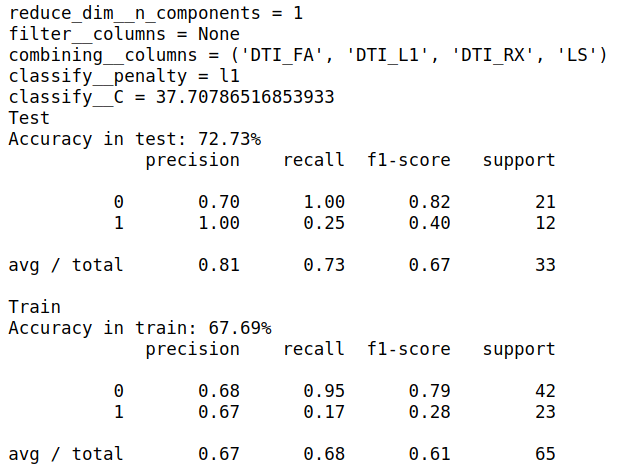
\includegraphics[width=0.5\textwidth]{figs/resultados/log_all.png}}
\caption{Resultado ejecución algoritmo Logistic Regression. Considerando todas las matrices.}
\label{figure:logall}
\end{figure}

\begin{figure}[H]
\centering
\fbox{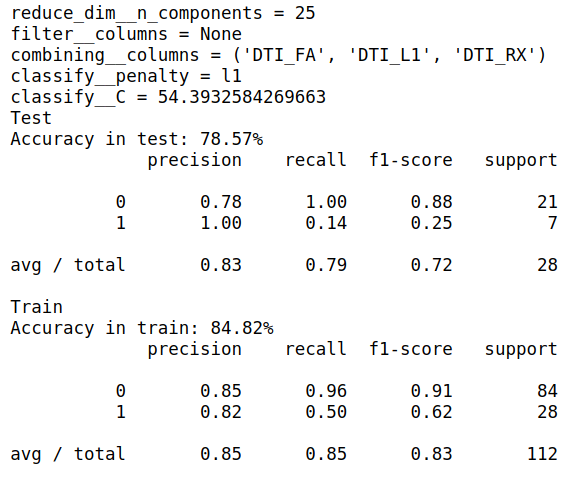
\includegraphics[width=0.5\textwidth]{figs/resultados/log_dti.png}}
\caption{Resultado ejecución algoritmo Logistic Regression. Considerando sólo matrices \gls{dti}.}
\label{figure:logdti}
\end{figure}

\begin{figure}[H]
\centering
\fbox{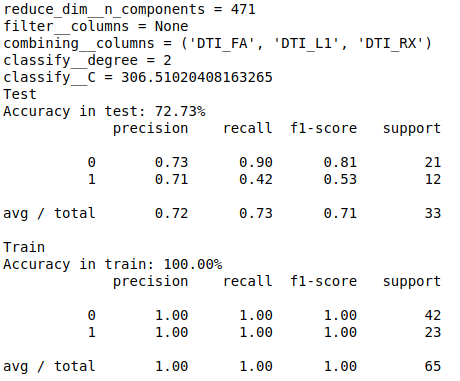
\includegraphics[width=0.5\textwidth]{figs/resultados/svm_all.png}}
\caption{Resultado ejecución algoritmo Support Vector Machine. Considerando todas las matrices.}
\label{figure:svmall}
\end{figure}

\begin{figure}[H]
\centering
\fbox{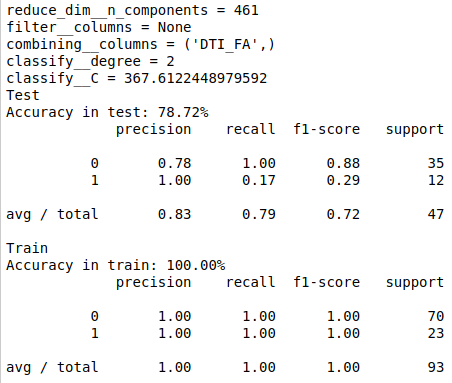
\includegraphics[width=0.5\textwidth]{figs/resultados/svm_dti.png}}
\caption{Resultado ejecución algoritmo Support Vector Machine. Considerando sólo matrices \gls{dti}.}
\label{figure:svmdti}
\end{figure}

\begin{figure}[H]
\centering
\fbox{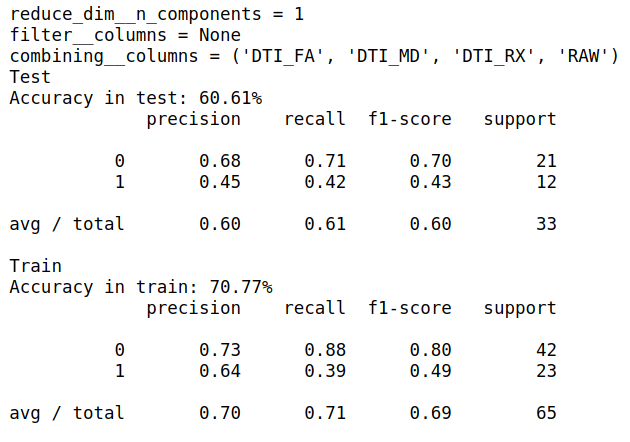
\includegraphics[width=0.5\textwidth]{figs/resultados/bayes_all.png}}
\caption{Resultado ejecución algoritmo Gaussian Naive Bayes. Considerando todas las matrices.}
\label{figure:bayesall}
\end{figure}

\begin{figure}[H]
\centering
\fbox{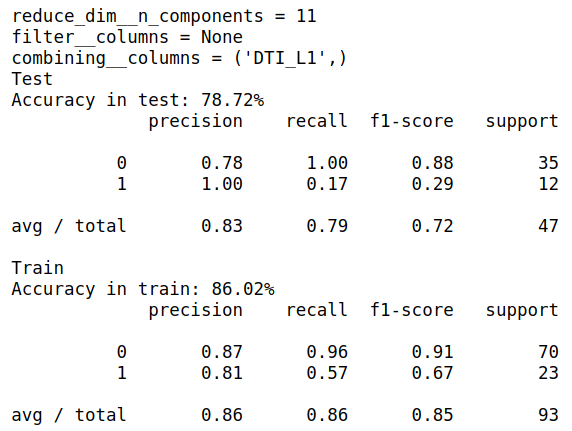
\includegraphics[width=0.5\textwidth]{figs/resultados/bayes_dti.png}}
\caption{Resultado ejecución algoritmo Gaussian Naive Bayes. Considerando sólo matrices \gls{dti}.}
\label{figure:bayesdti}
\end{figure}

\begin{figure}[H]
\centering
\fbox{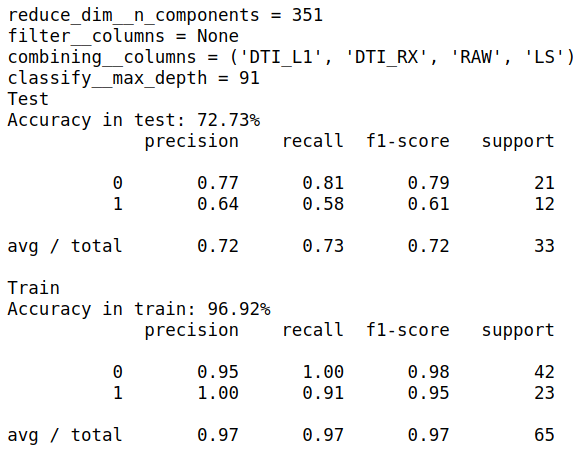
\includegraphics[width=0.5\textwidth]{figs/resultados/forest_all.png}}
\caption{Resultado ejecución algoritmo Random Forest Classifier. Considerando todas las matrices.}
\label{figure:forestall}
\end{figure}

\begin{figure}[H]
\centering
\fbox{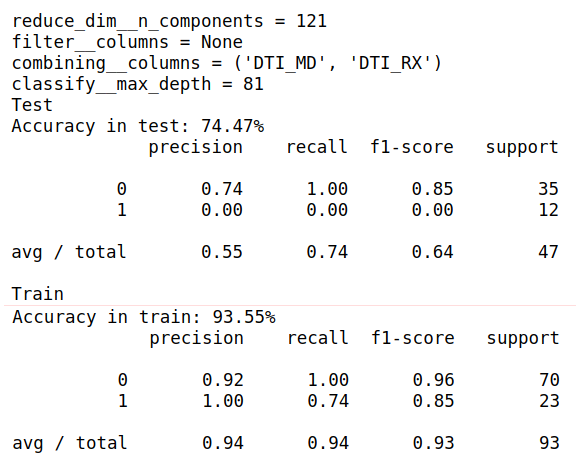
\includegraphics[width=0.5\textwidth]{figs/resultados/forest_dti.png}}
\caption{Resultado ejecución algoritmo Random Forest Classifier. Considerando sólo matrices \gls{dti}.}
\label{figure:forestdit}

\end{figure}
\begin{figure}[H]
\centering
\fbox{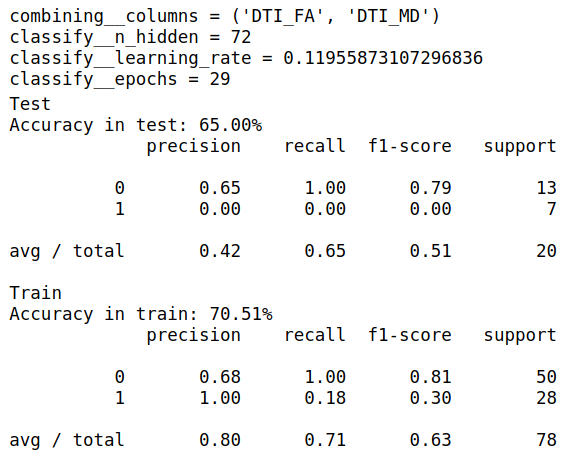
\includegraphics[width=0.5\textwidth]{figs/resultados/ann_all.png}}
\caption{Resultado ejecución algoritmo Artificial Neural Network. Considerando todas las matrices.}
\label{figure:annall}
\end{figure}

\begin{figure}[H]
\centering
\fbox{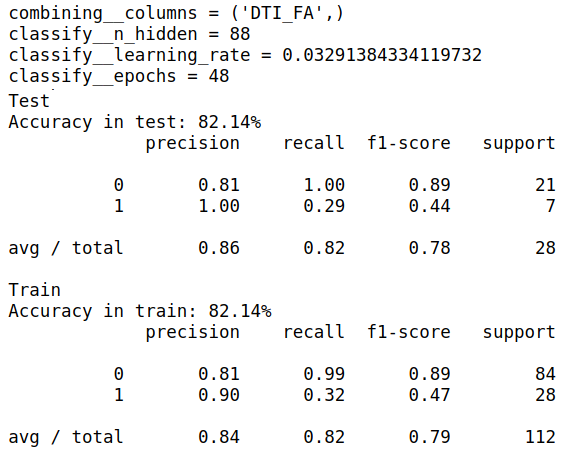
\includegraphics[width=0.5\textwidth]{figs/resultados/ann_dti.png}}
\caption{Resultado ejecución algoritmo Artificial Neural Network. Considerando sólo matrices \gls{dti}.}
\label{figure:anndti}
\end{figure}

La precisión es la habilidad del clasificador etiquetar correctamente los valores dentro de su grupo. La exhaustividad en cambio es la habilidad para acertar con las etiquetas en todo el conjunto. Por ejemplo, si disponemos de 10 ejemplares de donde 3 son del tipo A y 7 son del tipo B. A través de nuestro modelo obtenemos 5 elementos del tipo A pero sólo 2 han sido correctamente etiquetados, entonces nuestra precisión sería 2/3 y la exhaustividad 2/10. La medida-F1 engloba las otras dos siendo un valor único ponderado de la precisión y la exhaustividad. Su valor se calcula con la siguiente fórmula: 

$$F_1 = \frac{2}{\tfrac{1}{\mathrm{recall}} + \tfrac{1}{\mathrm{precision}}} = 2 \cdot \frac{\mathrm{precision} \cdot \mathrm{recall}}{\mathrm{precision} + \mathrm{recall}}$$

Aunque en este trabajo nos hemos centrado en una mejor ``accuracy'' pero igualmente, dependiendo de la finalidad de los experimentos se pueden ajustar para que la selección de los parámetros de la configuración tuviese como meta alguno de éstos.



% EPÍLOGO
\part{Epílogo}
\null\vfill
\chapter{Conclusiones}
\label{chapter:conclusiones}

\section{Experimentos}
La obtención de unos algoritmos que lograron unos resultados satisfactorios ha sido una ardua labor. Los problemas con el sobreajuste de los modelos (ver \ref{section:sobreajuste} siempre ha estado presente, en gran parte, debido al poco número de ejemplares con los que se dispone para el entrenamiento y la estrecha relación de los índices del tensor. Además, también ha causado que no todos los algoritmos respondieran  como se esperaba, ni siquiera tras buscar intensamente una configuración apropiada. 

Los algoritmos más simples han proporcionado unos mejores resultados y apenas eran propicios al sobreajuste. En cambio, cuando se aumentó la complejidad de los algoritmos, los resultados ya no eran tan satisfactorios. Por ejemplo, se intentó incrementar el número de capas ocultas en la ``Artificial Neural Network'' pero todos los resultados empeoraron notablemente. Por este motivo, se han descartado un gran número de algoritmos que no lograban estimar  las clases que representan las disfunciones cognitivas.

Finalmente se han seleccionado cinco modelos que han dado una respuesta muy esperanzadora. Como se puede ver en la tabla resumen \ref{table:resultados}, tres de los cinco han superado un acierto del 70\% al introducir todas las matrices de conectividad en el modelo de predicción de  la variable clínica (rendimiento cognitivo). Cuando se han usado solamente las matrices relacionadas con el tensor de difusión (índices sensibles a la microestructura del tejido subyacente), los resultados han mejorado considerablemente, llegando a una predicción del 75\% e incluso superando el 80\% en algunos casos. Esto ocurre también cuando buscamos una mejor configuración, como se ven en las imágenes 
\ref{figure:logall}, 
\ref{figure:svmall}, 
\ref{figure:bayesall}, 
\ref{figure:forestall} y
\ref{figure:annall}, donde se muestran las configuraciones de los modelos que dan mejores resultados.  A pesar de contar con todas las matrices de conectividad para la predicción del rendimiento cognitivo, el mejor modelo de predicción incluye únicamente a las matrices \gls{dti}. Señalando que estos datos son quizás los más sensibles para la manifestación de la disfunción cognitiva en los pacientes con \gls{em}.

Estos resultados, a pesar de ser convincentes, no pueden darse como definitivos ya que la búsqueda de los parámetros no ha sido posible ejecutarla completamente con todas las combinaciones posibles. Dado el elevado número de posibles combinaciones de los hiperparámentros, es inviable ejecutar todas ellas con el sistema disponible. Por ello se ha seleccionado la configuración entre 150 combinaciones aleatorias. Por otra parte, se aprecia claramente la importancia de los índices \gls{dti} sobre el resto y cómo éstas pueden son una fuente de datos válida para la estimación de las disfunciones cognitivas.

\section{Proyecto de investigación}
La realización de este trabajo ha sido un gran reto personal. Es la primera vez que me enfrento a un trabajo de investigación y, a la vez, a un ejercicio relacionado con el aprendizaje automático en el ámbito clínico. Todo esto conjuntamente con las lecciones aprendidas durante la realización del trabajo y los resultados obtenidos me han proporcionado experiencia muy positiva y enriquecedora.

La primera dificultad encontrada durante este trabajo fue la ``compresión del negocio''. Los datos usados en este trabajo tienen tras de sí múltiples investigaciones, teorías y técnicas que ha sido necesarias para poder comprender y trabajar con los datos. El conocimiento adquirido durante esta fase inicial ha sido de gran utilidad a lo largo de la ejecución del proyecto.

Uno de los mayores retos durante el proceso de investigación ha sido la búsqueda de algoritmos capaces de dar respuesta a las objetivos planteados dado el gran número de algoritmos disponibles y todas las opciones que el aprendizaje automático provee. Además, siempre hay que considerar los requerimientos y el tiempo de cómputo que los algoritmos necesitan. A pesar de las implementaciones óptimas ofrecidas por los  ``frameworks'', el hardware usado se ha visto a menudo incapaz de soportar la carga de trabajo en un tiempo razonable. Para lidiar en parte con este problema se optó por la búsqueda aleatoria de la configuración de los algoritmos seleccionados. 

En definitiva, el objetivo inicial planteado para la superación del trabajo final de Máster de ciencia de datos ha sido cumplido. Los resultados obtenidos demuestran  cómo los algoritmos de aprendizaje automático pueden ayudar a la predicción del rendimiento cognitivo del paciente con \gls{em} a través de la cuantificación del volumen lesional y la microestructura de la red cerebral.


\chapter{Trabajo Futuro}
\label{chapter:trabajofuturo}
Este trabajo de investigación se puede considerar como un primer paso para una investigación más profunda. La obtención de una cohorte mayor y la introducción de nuevos datos relacionados con la disfunción cognitiva, como por ejemplo medidas de atrofia, podrían mejorar la eficiencia de las técnicas de aprendizaje automático. 

En primer lugar, sería muy interesante comprobar los resultados obtenidos con una fuente de datos más amplia y poder investigar la configuración óptima de los algoritmos con más profundidad. 

Por falta de tiempo se han quedado sin ejecutar algunas propuestas para la reducción de la dimensionalidad, por ejemplo \gls{csp}, y también técnicas que combinan clasificadores sencillos para obtener un más complejo (bagging y stacking). Experimentos con estas técnicas también podrían producir resultados interesantes.


\addcontentsline{toc}{chapter}{Bibliografía}
% bibliografía
\begin{flushright}

\bibliographystyle{IEEEtran} % IEEEtran or alphadin??

\bibliography{mendeley_v2}
\end{flushright}





\end{document}